\chapter{Introduction, apprentissage supervisé, bornes}

\myminitoc

\sect{Introduction}

\paragraph{Qu'est ce que le machine learning ?}
Le machine learning est le développement d'algorithmes qui apprennent tout seul à partir de données. On distingue deux catégorie :
\begin{itemize}
	\item L'apprentissage supervisé : qui apprend avec des données étiquetées afin de faire de la classification, de la régression ou encore de la hiérarchisation.
	\item  L'apprentissage non supervisé : qui trouve la structure d'un jeu de données afin de faire du clustering ou de la réduction de dimensions.
\end{itemize}
Les applications principales du machine learning sont alors la vision par ordinateur, la robotique, la reconnaissance vocale, le traitement du langage, etc ...

\sect{Apprentissage supervisé}

\DEF{
	Dans la suite on utilisera les notations suivantes :
	\begin{itemize}
		\item On pose $\bm{S = \{ z_i = (x_i, y_i) \}_{i = 1}^m}$ un ensemble de $\bm{m}$ exemples d'entraînement indépendants et identiquement distribués selon une une distribution inconnue $\bm{\dist}$ sur l'espace $\bm{\Z = \X \times \Y}$.
		\item Les valeurs $x_i \in \bm{\X}$ sont généralement des vecteurs de $\R^d$ dont les composantes sont appelées les \textbf{features}.
		\item Les valeurs $y_i \in \bm{\Y}$ se trouvent dans l'ensemble discret des \textbf{classes/étiquettes} (typiquement $\Y = \{ -1, +1 \}$ en classification binaire) ou dans un ensemble continue dans le cas de régressions.
		\item Finalement on cherche une \textbf{fonction cible} $\bm{f}$ tel que $\bm{\forall (x, y) \in \dist, \, y = f(x)}$.
	\end{itemize}
}

\DEF{
	Un \textbf{algorithme d'apprentissage supervisé} $\bm{L}$ prend en entrée $S$ et retourne un modèle ou une classification $\bm{h \in \Hyp}$ le plus proche possible de $f$.
}

\exe
Si on prend pour $f$ la fonction qui retourne {\color{red}$y = +1$} si $x_1^2 + x_2^2 < R^2$ et {\color{blue}$y = -1$} sinon, alors voici le résultat que l'on peut obtenir :
\begin{center}
	\begin{tikzpicture}[thick, scale=1.2]
		\draw[greenTikz, opacity=0.4] (0, 0) circle (1);
		\node[greenTikz] at (0.8, -0.9) {$f$};
		\draw[blue] (-2, 0) -- (2, 0) node[below left, black] {$x_1$};
		\draw[blue] (0, -2) -- (0, 1.8) node[above, black] {$x_2$};
		\draw[fill, red] (0.2, 0.7) circle (0.08);
		\draw[fill, red] (-0.4, -0.5) circle (0.08);
		\draw[fill, red] (0.2, -0.3) circle (0.08);
		\draw[fill, red] (-0.3, 0.3) circle (0.08);
		\draw[fill, red] (0.4, 0.2) circle (0.08);
		\draw[orange, very thick] (0.2, -1.5)
			.. controls (-0.5, -1) and (-1, -0.2) .. (-0.95, -0.05)
			.. controls (-1, 0.2) and (-0.4, 1) .. (0.3, 0.9)
			.. controls (0.9, 0.75) and (1, 0) .. (1.1, -0.4)
			.. controls (1.15, -0.6) and (1.05, -1.2) .. (0.8, -1.5) node[below] {$h$};
		\draw[fill, blue] (-1.1, 0.3) circle (0.08);
		\draw[fill, blue] (-1.2, -0.1) circle (0.08);
		\draw[fill, blue] (-1.3, -0.5) circle (0.08);
		\draw[fill, blue] (-1.2, -0.8) circle (0.08);
		\draw[fill, blue] (-0.8, -1.2) circle (0.08);
		\draw[fill, blue] (-0.3, -1.5) circle (0.08);
		\draw[fill, blue] (-0.6, 1) circle (0.08);
		\draw[fill, blue] (-0.9, 0.8) circle (0.08);
		\draw[fill, blue] (-0.95, 1.2) circle (0.08);
		\draw[fill, blue] (-0.2, 1.3) circle (0.08);
		\draw[fill, blue] (0.3, 1.1) circle (0.08);
		\draw[fill, blue] (0.7, 0.9) circle (0.08);
		\draw[fill, blue] (1.1, 0.5) circle (0.08);
		\draw[fill, blue] (1.3, 0.1) circle (0.08);
		\draw[fill, blue] (1.3, -0.4) circle (0.08);
		\draw[fill, blue] (1.25, -1.2) circle (0.08);
	\end{tikzpicture}
\end{center}
Ici $h$ convient aux données d'entraînement mais n'est toujours pas bon pour la généralisation.

\paragraph{Conjecture}
Plus l'ensemble $S$ sera grand, plus la fonction $h$ sera proche de $f$.

\paragraph{Malédiction de la dimensionnalité}
Quand le nombre de features augmente, le nombre $m$ d'exemples d'entraînement nécessaires pour généralisé de manière assez précise augmente exponentiellement.

\DEF{
	En statistiques, l'\textbf{overfitting} est le phénomène où le modèle obtenu est trop complexe. Il peu avoir trop de degrés de liberté par exemple. En revanche l'\textbf{underfitting} est lorsque le modèle n'arrive pas à trouver la tendance des données. 
}

\subs{Risque et fonction de perte}

\DEF{
	En théorie, on aime considéré la meilleurs hypothèse $h^* \in \Hyp$. En se donnant une \textbf{fonction de perte} $l : \Hyp \times \Z \rightarrow \R$ mesurant le degré d'accord entre $h(x)$ et $y$, le \textbf{vrai risque} ou \textbf{erreur de généralisation} $\trisk(h)$ est défini ainsi :
	$$ \trisk(h) = \E_{z \sim \dist} l(h, z) = \int_z f_\dist(z) l(h, z)$$
	$$ h^* = \argmin_{h \in \Hyp} \trisk(h) $$
	\vspace{-5mm}
}

Malheureusement, $\trisk(h)$ ne peut pas être calculé car $\dist$ est inconnu. On peut seulement calculé le \textbf{risque empirique} sur $S$. C'est à dire :
$$ \erisk(h) = \E_{z \sim S} l(h, z) = \frac{1}{m} \sum_{i = 1}^{m} l(h, z_i) $$
Ainsi le but de l'algorithme d'apprentissage supervisé est de trouver le modèle $\displaystyle h = \argmin_{h_i \in \Hyp} \erisk(h_i)$.

\exe
La fonction de perte la plus naturelle pour la classification binaire est le 0/1 loss.
$$ l_{0/1}(h, z) = \left\{ \begin{array}{ll}
	1 & \text{si } yh(x) < 0 \\
	0 & \text{sinon}
\end{array}
\right. $$
Ainsi $\mathcal{R}^{l_{0/1}}(h)$ est la proportion de mauvaises prédictions. \\
Malheureusement, à cause de la non-convexité et de la non-différentiabilité de cette fonction de perte, minimiser, ou même minimiser approximativement $\mathcal{\hat{R}}^{l_{0/1}}(h)$ est un problème NP-difficile.

\paragraph{Fonctions de perte usuelles} Pour cette raison, on utilise généralement les fonctions de perte convexes suivante :
\begin{itemize}
	\item La \textbf{perte exponentielle} (utilisée en boosting) : $l_{exp}(h, z) = e^{-yh(x)}$
	\item La \textbf{perte logistique} (utilisée en régression logistique) : $l_{log}(h, z) = \ln(1 + e^{-yh(x)})$
	\item La \textbf{perte charnière} (utilisée en SVM) : $l_{hinge}(h, z) = \max(0, 1 - yh(x))$
\end{itemize}
\begin{center}
	\begin{tikzpicture}[yscale=1.25, xscale=1.65, thick]
		\draw (-2, -0.5) node[below] {-2} -- (2, -0.5) node[below] {2};
		\draw (-2, -0.5) node[left] {-0.5} -- (-2, 3.5) node[left] {3.5};
		\draw (0, -0.5) node[] {\tiny |} node[below] {0};
		\draw (-2, 1.5) node[] {\tiny -} node[left] {1.5};
		\draw (-2, 1) node[left] {1} -- (0, 1) -- (0, 0) -- (2, 0);
		\draw[red] (-2, 3) -- (1, 0) -- (2, 0);
		\draw[domain=-1.25:2, smooth, variable=\x, blue] plot ({\x}, {exp(-\x)});
		\draw[domain=-2:2, smooth, variable=\x, greenTikz] plot ({\x}, {ln(1 + exp(-\x))});
		\draw (1.8, 3.3) -- (1.3, 3.3) node[left] {\footnotesize 0/1 loss};
		\draw[red] (1.8, 3) -- (1.3, 3) node[left] {\footnotesize hinge loss};
		\draw[greenTikz] (1.8, 2.7) -- (1.3, 2.7) node[left] {\footnotesize logistic loss};
		\draw[blue] (1.8, 2.4) -- (1.3, 2.4) node[left] {\footnotesize exponential loss};
	\end{tikzpicture}
\end{center}

\subs{Minimisation de risque régularisée}

Trop entraîner l'algorithme sur les données d'entraînement $S$ peut conduire à une mémorisation et à l'overfitting. Le modèle devient compliqué et on risque d'avoir une mauvaise généralisation. Le principe du \textbf{rasoir d'Occam} est "le plus simple est le mieux". Pour appliquer ce principe, on essaye de minimiser les paramètres du modèle. \\
On va donc minimiser le \textbf{risque empirique régularisé} :
$$ \min_{h \in \Hyp} \erisk(h) + \lambda \| h \| $$
On pénalise alors les hypothèses avec une forte norme.

\DEF{
	La norme $l_p$ d'un vecteur $\theta$ d'un espace à $d$ dimensions est défini comme suit :
	\vspace*{-3mm}
	$$ \| \theta \|_p = \left( \sum_{i = 1}^d |\theta_i|^p \right)^{\frac{1}{p}} $$
	\vspace{-5mm}
}

\begin{center}
	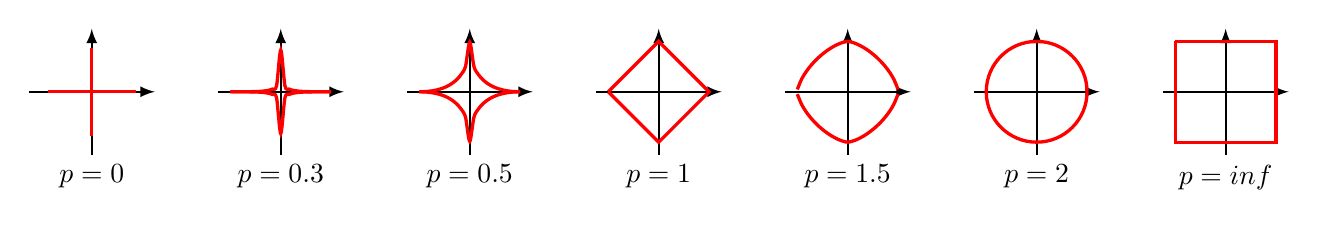
\begin{tikzpicture}[thick, >={latex}, scale=0.8]
		\draw[->] (0, 0) -- (2, 0);
		\draw[->] (1, -1) node[below] {$p=0$} -- (1, 1);
		\draw[red, very thick] (0.3, 0) -- (1.7, 0);
		\draw[red, very thick] (1, -0.7) -- (1, 0.7);
		
		\draw[->] (3, 0) -- (5, 0);
		\draw[->] (4, -1) node[below] {$p=0.3$} -- (4, 1);
		\draw[domain=-1:1, smooth, variable=\x, red, very thick]
			plot ({0.8*\x+4}, {0.8 * max(0.01, 1 - abs(\x)^0.3)^(1/0.3)});
			\draw[domain=-1:1, smooth, variable=\x, red, very thick]
			plot ({0.8*\x+4}, {-0.8 * max(0.01, 1 - abs(\x)^0.3)^(1/0.3)});
			
		\draw[->] (6, 0) -- (8, 0);
		\draw[->] (7, -1) node[below] {$p=0.5$} -- (7, 1);
		\draw[domain=-1:1, smooth, variable=\x, red, very thick]
			plot ({0.8*\x+7}, {0.8 * max(0.01, 1 - abs(\x)^0.5)^(1/0.5)});
		\draw[domain=-1:1, smooth, variable=\x, red, very thick]
			plot ({0.8*\x+7}, {-0.8 * max(0.01, 1 - abs(\x)^0.5)^(1/0.5)});
		
		\draw[->] (9, 0) -- (11, 0);
		\draw[->] (10, -1) node[below] {$p=1$} -- (10, 1);
		\draw[red, very thick] (9.2, 0) -- (10, 0.8) -- (10.8, 0) -- (10, -0.8) -- (9.2, 0);
		
		\draw[->] (12, 0) -- (14, 0);
		\draw[->] (13, -1) node[below] {$p=1.5$} -- (13, 1);
		\draw[domain=-1:1, smooth, variable=\x, red, very thick]
			plot ({0.8*\x+13}, {0.8 * max(0.01, 1 - abs(\x)^1.5)^(1/1.5)});
		\draw[domain=-1:1, smooth, variable=\x, red, very thick]
			plot ({0.8*\x+13}, {-0.8 * max(0.01, 1 - abs(\x)^1.5)^(1/1.5)});
		
		\draw[->] (15, 0) -- (17, 0);
		\draw[->] (16, -1) node[below] {$p=2$} -- (16, 1);
		\draw[red, very thick] (16, 0) circle (0.8);
		
		\draw[->] (18, 0) -- (20, 0);
		\draw[->] (19, -1) node[below] {$p=inf$} -- (19, 1);
		\draw[red, very thick] (18.2, 0.8) -- (19.8, 0.8) -- (19.8, -0.8) -- (18.2, -0.8) -- (18.2, 0.8);
	\end{tikzpicture}
\end{center}

La norme $l_2$ est utilisée pour réduire les risques d'overfitting en réduisant les plus grandes valeurs du modèle. La norme $l_1$, elle permet d'obtenir des modèles creux, c'est à dire avec peu de features.

\exe
Considérons le problème suivant : \vspace{-1mm}
$$ \min_{\theta \in \R^d} \frac{1}{2} \theta^\trans \theta - \theta^\trans x + \lambda \| \theta \|_2^2 $$
Si $\lambda = 0$, alors : \vspace{-1mm}
$$ \dfrac{\partial \frac{1}{2} \theta^\trans \theta - \theta^\trans x}{\partial \theta_j} = 0 \Rightarrow \theta_j - x_j = 0 \Rightarrow \fbox{$\theta_j = x_j$} $$
Si $\lambda \neq 0$, alors : \vspace{-2mm}
$$ \dfrac{\partial \frac{1}{2} \theta^\trans \theta - \theta^\trans x  + \lambda \| \theta \|_2^2}{\partial \theta_j} = 0 \Rightarrow \theta_j - x_j +2\lambda \theta_j = 0 \Rightarrow \fbox{$\theta_j = \dfrac{x_j}{1 + 2\lambda}$} $$
\begin{center}
	\begin{tikzpicture}[>={latex}, thick]
	\draw[->] (-1, 0) -- (5, 0);
	\draw[->] (0, -1) -- (0, 3.5);
	\draw (3, 0) node {\tiny |} node[below] {3};
	\draw (0, 2) node {\tiny -} node[left] {2};
	\draw[fill] (3, 2) circle (0.05) node[below] {$x$};
	\draw[fill=greenTikz, fill opacity=0.5, very thick] (3, 2) circle (1.4^0.5);
	\draw[very thick] (3, 2) circle (1) circle (0.6^0.5) circle (0.2^0.5);
	\node[color=red] at (1, -0.6) {$\lambda = 0$};
	
	\draw[->] (7, 0) -- (13, 0);
	\draw[->] (8, -1) -- (8, 3.5);
	\draw (11, 0) node {\tiny |} node[below] {3};
	\draw (8, 2) node {\tiny -} node[left] {2};
	\draw[fill] (11, 2) circle (0.05) node[below] {$x$};
	\draw[fill=greenTikz, fill opacity=0.5, very thick] (9, 0.67) circle (0.47^0.5);
	\draw[very thick] (9, 0.67) circle (0.33^0.5) circle (0.2^0.5) circle (0.07^0.5);
	\node[color=red] at (9, -0.6) {$\lambda = 1$};
	\end{tikzpicture}
\end{center}

\exe
Maintenant on peut prendre la norme $l_1$ pour constater qu'elle engendre bien un vecteur de paramètres creux.
$$ \min_{\theta \in \R^d} \frac{1}{2} \theta^\trans \theta - \theta^\trans x + \lambda \| \theta \|_1 $$
Si $\lambda = 0$, on a vu que $\theta^* = x$. \\
En revanche si $\lambda > 0$, on considère la dérivée partielle à $\theta_j = 0^+$, et à $\theta_j = 0^-$ :
$$ g_+^j = \lambda - x_j \qquad g_-^j = - \lambda - x_j $$
Or $\theta_j^* = 0$ si et seulement si $g_+^j \geqslant 0$ et $g_-^j \leqslant 0$. C'est à dire si $x_j \geqslant \lambda$ et $x_j \leqslant -\lambda$. \\
Donc si $|x_j| \leqslant \lambda$ alors $\theta_j^* = 0$.
\begin{center}
	\begin{tikzpicture}[>={latex}, thick, scale=0.8]
	\draw[->] (-1, 0) -- (5, 0);
	\draw[->] (0, -1) -- (0, 3.5);
	\draw (3, 0) node {\tiny |} node[below] {3};
	\draw (0, 2) node {\tiny -} node[left] {2};
	\node[color=red] at (1, -0.6) {$\lambda = 0$};
	\draw[fill] (3, 2) circle (0.05) node[below] {$x$};
	\draw[fill=greenTikz, fill opacity=0.5, very thick] (3, 2) circle (5^0.5);
	\draw[very thick] (3, 2) circle (3^0.5) circle (1);
	
	\draw[->] (7, 0) -- (13, 0);
	\draw[->] (8, -1) -- (8, 3.5);
	\draw (11, 0) node {\tiny |} node[below] {3};
	\draw (8, 2) node {\tiny -} node[left] {2};
	\draw[fill] (11, 2) circle (0.05) node[below] {$x$};
	\draw[fill, red] (9, 0) circle (0.05) node[above] {$\theta^*$};
	\node[color=red] at (12.4, 3) {$\lambda = 2$};
	\node[color=red] at (12.4, 2.5) {$\theta^*$ est creux};
	\draw[very thick, fill=greenTikz, fill opacity=0.5] (11.24, 0) arc (0:116.6:2.24);
	\draw[very thick, fill=greenTikz, fill opacity=0.5] (8, 2) arc (158:180:5.39);
	\draw[very thick, fill=greenTikz, fill opacity=0.5] (7.61, 0) arc (217:222.4:6.71);
	\draw[very thick, fill=greenTikz, fill opacity=0.5] (8, -0.47) arc (257.4:299.1:4.58);
	\draw[very thick] (10, 0) arc(0:180:1);
	\draw[very thick] (8, 0) arc(-104:-76:4.12);
	\draw[very thick] (10.73, 0) arc(0:125:3^0.5);
	\draw[very thick] (7.8, 0) arc(180:164:27^0.5);
	\draw[very thick] (7.8, 0) arc(217.6:220.5:43^0.5);
	\draw[very thick] (10.73, 0) arc(-66.6:-103:19^0.5);
	\fill[greenTikz, opacity=0.5] (11.24, 0) -- (8, 2) -- (7.61, 0) -- (8, -0.47);
	\end{tikzpicture}
\end{center}

\paragraph{Supprimer des groupes de features}
Voici des normes qui permettent de supprimer les features en groupe :
\begin{center}
	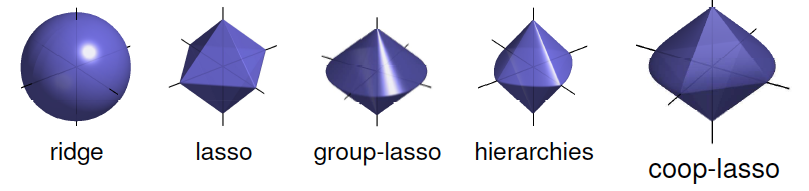
\includegraphics[scale=0.5]{group_sparse.png}
\end{center}
On considère $\{ \mathcal{G}_{k = 1}^K \}$ une partition de $\{ 1, \dots, d \}$. On peur alors définir les normes suivantes :
$$ \| \theta \|_{group} = \sum_{g \in \mathcal{G}} \left( \sum_{j \in g} \theta_j^2 \right)^{\frac{1}{2}} $$
$$ \| \theta \|_{coop} = \sum_{g \in \mathcal{G}} \left[ \left( \sum_{j \in g} [\theta_j]_+^2 \right)^{\frac{1}{2}} + \left( \sum_{j \in g} [\theta_j]_-^2 \right)^{\frac{1}{2}} \right] $$

\newpage
\subs{Contrepartie Biais/Variance}

D'où vient l'erreur de $h \in \Hyp$ ?
\begin{itemize}
	\item Du \textbf{biais inductif}. Rien ne garanti l'égalité entre l'espace cible des concepts $\mathcal{F}$ et la classe d'hypothèse que l'on a choisi $\Hyp$.
	\item De la \textbf{variance}. Comme l'ensemble d'entraînement est fini et choisi aléatoirement selon $\dist$, l'algorithme d'apprentissage ne retourne pas l'hypothèse optimale $h^*$ de $\Hyp$.
\end{itemize}

\begin{center}
	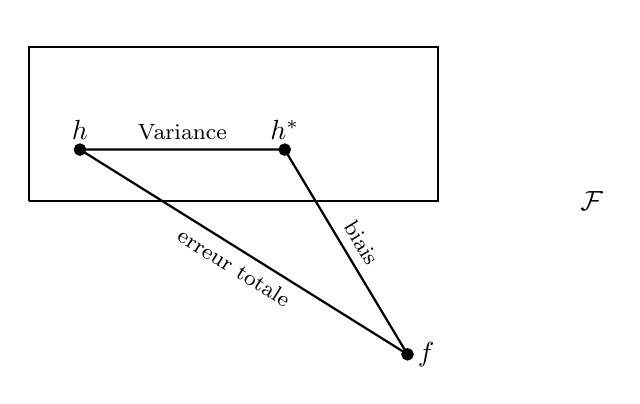
\begin{tikzpicture}[thick, scale=1.3]
		\draw (0, 0.5) -- (4, 0.5) -- (4, 2) -- node[above] {$\Hyp$} (0, 2) -- (0, 0.5);
		\node at (5.5, 0.5) {$\mathcal{F}$};
		\draw[fill] (0.5, 1) circle (0.05) node[above] {$h$}
			-- node[below, sloped] {\footnotesize erreur totale} (3.7, -1)
				circle (0.05) node[right] {$f$}
			-- node[above, sloped] {\footnotesize biais} (2.5, 1)
				circle (0.05) node[above] {$h^*$}
			-- node[above] {\footnotesize Variance} (0.5, 1);
	\end{tikzpicture}
\end{center}
$$ \trisk(h) \leqslant \text{Biais} + \text{Variance} $$
$$ \trisk(h) \leqslant \text{Biais inévitable} + \text{Biais évitable} + \text{Variance} $$
$$ \trisk(h) \leqslant {\color{red}\text{Erreur de Bayes}} + {\color{blue}\text{Biais évitable}} + {\color{blue}\text{Variance}} $$

\DEF{
	L'\textbf{erreur de Bayes} $\epsilon_B$ est le plus petit taux d'erreur pour une hypothèse $h$ :
	$$ \epsilon_B = \sum_i \int_{(x, y) \in R_i \times \bar{C_i}} P(C_i | x) p(x) dx $$
	Où $x$ est une instance avec $y$ pour étiquette et $R_i$ est la région que la fonction de classification $h$ classifie comme $C_i$.
}
\begin{center}
	C'est un $\ll$ sept $\gg$ ou un $\ll$ un $\gg$ ? \\
	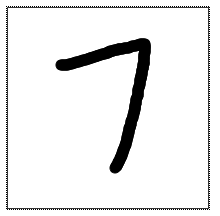
\includegraphics[scale=0.4]{one_seven.png}
\end{center}

\newpage
\paragraph{Variance}
$h$ va converger vers $h^*$ si on augmente le nombre d'exemples $m$.
\begin{center}
	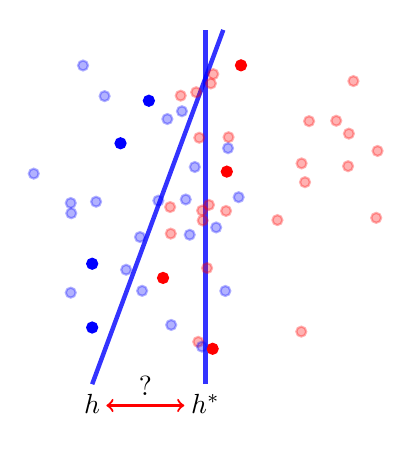
\begin{tikzpicture}[thick, scale=0.9]
		\draw[ultra thick, blue, opacity=0.8] (0, -2.5) -- (0, 2.5);
		\draw[ultra thick, blue, opacity=0.8] (-1.6, -2.5) -- (0.25, 2.5);
		\node[below] at (-1.6, -2.5) {$h$};
		\node[below] at (0, -2.5) {$h^*$};
		\draw[<->, red] (-0.3, -2.8) -- node[black, above] {?} (-1.4, -2.8);
		\draw[fill, red] (0.1, -2) circle (0.07);
		\draw[fill, red] (-0.6, -1) circle (0.07);
		\draw[fill, red] (0.3, 0.5) circle (0.07);
		\draw[fill, red] (0.5, 2) circle (0.07);
		\draw[fill, red, opacity=0.3] (-0.5, 0) circle (0.07);
		\draw[fill, red, opacity=0.3] (0.3243, 0.9859) circle (0.07);
		\draw[fill, red, opacity=0.3] (-0.08914, 0.978) circle (0.07);
		\draw[fill, red, opacity=0.3] (2.427, 0.7918) circle (0.07);
		\draw[fill, red, opacity=0.3] (1.4609, 1.212) circle (0.07);
		\draw[fill, red, opacity=0.3] (1.3548, 0.6159) circle (0.07);
		\draw[fill, red, opacity=0.3] (1.403, 0.351) circle (0.07);
		\draw[fill, red, opacity=0.3] (-0.351, 1.57183) circle (0.07);
		\draw[fill, red, opacity=0.3] (0.10869, 1.876) circle (0.07);
		\draw[fill, red, opacity=0.3] (-0.13232, 1.62) circle (0.07);
		\draw[fill, red, opacity=0.3] (0.048154, 0.0303) circle (0.07);
		\draw[fill, red, opacity=0.3] (0.0214, -0.861) circle (0.07);
		\draw[fill, red, opacity=0.3] (-0.10329, -1.902) circle (0.07);
		\draw[fill, red, opacity=0.3] (-0.049, -0.0497) circle (0.07);
		\draw[fill, red, opacity=0.3] (1.3507, -1.7576) circle (0.07);
		\draw[fill, red, opacity=0.3] (-0.4912, -0.3749) circle (0.07);
		\draw[fill, red, opacity=0.3] (1.0138, -0.184) circle (0.07);
		\draw[fill, red, opacity=0.3] (2.0108, 0.5766) circle (0.07);
		\draw[fill, red, opacity=0.3] (2.0224, 1.0361) circle (0.07);
		\draw[fill, red, opacity=0.3] (0.0751, 1.7442) circle (0.07);
		\draw[fill, red, opacity=0.3] (2.0863, 1.7777) circle (0.07);
		\draw[fill, red, opacity=0.3] (-0.0409, -0.1897) circle (0.07);
		\draw[fill, red, opacity=0.3] (0.2889, -0.0546) circle (0.07);
		\draw[fill, red, opacity=0.3] (2.4079, -0.1523) circle (0.07);
		\draw[fill, red, opacity=0.3] (1.8439, 1.2179) circle (0.07);
		
		\draw[fill, blue] (-0.8, 1.5) circle (0.07);
		\draw[fill, blue] (-1.2, 0.9) circle (0.07);
		\draw[fill, blue] (-1.6, -0.8) circle (0.07);
		\draw[fill, blue] (-1.6, -1.7) circle (0.07);
		\draw[fill, blue, opacity=0.3] (-1.9025, 0.0568) circle (0.07);
		\draw[fill, blue, opacity=0.3] (-0.2239, -0.3909) circle (0.07);
		\draw[fill, blue, opacity=0.3] (-0.6662, 0.0906) circle (0.07);
		\draw[fill, blue, opacity=0.3] (0.4667, 0.1391) circle (0.07);
		\draw[fill, blue, opacity=0.3] (-0.0517, -1.9698) circle (0.07);
		\draw[fill, blue, opacity=0.3] (-1.1208, -0.8846) circle (0.07);
		\draw[fill, blue, opacity=0.3] (0.1495, -0.2879) circle (0.07);
		\draw[fill, blue, opacity=0.3] (-2.4247, 0.4716) circle (0.07);
		\draw[fill, blue, opacity=0.3] (-1.9027, -1.2081) circle (0.07);
		\draw[fill, blue, opacity=0.3] (-1.4246, 1.5652) circle (0.07);
		\draw[fill, blue, opacity=0.3] (-1.729, 1.9974) circle (0.07);
		\draw[fill, blue, opacity=0.3] (-0.5392, 1.2422) circle (0.07);
		\draw[fill, blue, opacity=0.3] (0.3168, 0.8305) circle (0.07);
		\draw[fill, blue, opacity=0.3] (-0.2799, 0.1071) circle (0.07);
		\draw[fill, blue, opacity=0.3] (-1.5449, 0.0752) circle (0.07);
		\draw[fill, blue, opacity=0.3] (-1.8949, -0.0877) circle (0.07);
		\draw[fill, blue, opacity=0.3] (-0.9253, -0.423) circle (0.07);
		\draw[fill, blue, opacity=0.3] (0.279, -1.1842) circle (0.07);
		\draw[fill, blue, opacity=0.3] (-0.152, 0.5651) circle (0.07);
		\draw[fill, blue, opacity=0.3] (-0.8953, -1.1821) circle (0.07);
		\draw[fill, blue, opacity=0.3] (-0.3335, 1.352) circle (0.07);
		\draw[fill, blue, opacity=0.3] (-0.4852, -1.6634) circle (0.07);
	\end{tikzpicture}
\end{center}

\paragraph{Biais évitable}
La distance entre l'espace $\Hyp$ et $f$ va diminuer si on augmente l'expressivité de $h$ et notamment en augmentant la dimension.

\paragraph{Conclusion}
Malheureusement, augmenter la dimension augmente aussi la variance. Il faut donc trouver un bon compromis sur la dimension pour réduire le biais sans trop augmenter la variance.
\begin{center}
	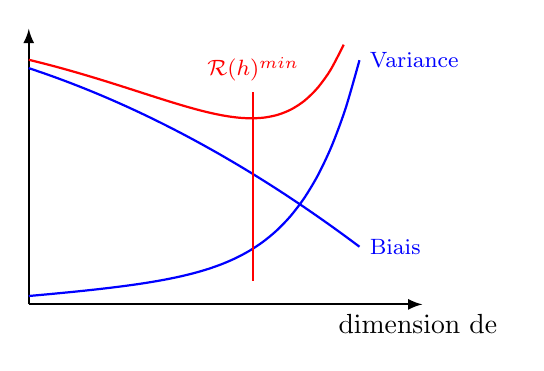
\begin{tikzpicture}[thick, >={latex}]
		\draw[->] (0, 0) -- (5, 0) node[below] {dimension de $\Hyp$};
		\draw[->] (0, 0) -- (0, 3.5);
		\draw[domain=0:4.2, smooth, variable=\x, blue]
			plot ({\x}, {3 - \x * (0.33 + 0.05 * \x)})
			node[right] {\footnotesize Biais};
		\draw[domain=0:4.2, smooth, variable=\x, blue]
			plot ({\x}, {0.1 + 0.08 * \x + 0.42 * exp(1.44 * \x - 4.2)})
			node[right] {\footnotesize Variance};
		\draw[domain=0:4, smooth, variable=\x, red]
			plot ({\x}, {3.1 - \x * (0.25 + 0.05 * \x) + 0.42 * exp(1.44 * \x - 4.2)});
		\draw[red] (2.85, 0.3) -- (2.85, 2.7) node[above] {\footnotesize $\trisk(h)^{min}$};
	\end{tikzpicture}
\end{center} 

\subs{Bornes de généralisation}

\paragraph{But}
Notre objectif est d'obtenir des bornes \textbf{PAC (Probably Approximately Correct)} de la forme suivante : Avec probabilité $1 - \delta$
$$ \begin{array}{lll}
	\trisk(h) & \leqslant & \erisk(h) + \gamma \\
	 & \leqslant & \erisk(h^*) + 2 \gamma \qquad \text{(car } h = \argmin_{h_i \in \Hyp} \erisk(h_i)) \\
	 & \leqslant & (\trisk(h^*) + \gamma) + \gamma \\
	 & \leqslant & \trisk(h^*) + 2 \gamma
\end{array} $$

La théorie de la convergence uniforme nous donne des garanties pour les hypothèses $h \in \Hyp$. La question que l'on se pose est : Sous quelle conditions (sur le nombre minimum d'exemples d'entraînement requis) peut-on obtenir des bornes PAC valides ? \\
On va considérer deux situations. La première est celle où $|\Hyp| = k$ est fini. La seconde est celle où $\Hyp$ est infini.

\subsubs{Convergence uniforme - Cas fini}

On commence par rappeler le lemme suivant: \vspace{3mm}
\PROP[ (Inégalité de Hoeffding)]{
	Soit $Z_1, \dots, Z_m$ $m$ variables i.i.d suivant des loi de Bernoulli d'espérance $\phi$. On pose la variable $\hat{\phi} = \frac{1}{m} \sum_{i = 1}^m Z_i$ et on considère $\gamma > 0$. Alors : \vspace{-2mm}
	$$ \Pp(|\hat{\phi} - \phi| > \gamma) \leqslant 2 \exp(-2 \gamma^2 m) $$
	\vspace{-9mm}
}
\vspace{2mm}

On considère alors l'espace $\Hyp = \{ h_1, \dots, h_k \}$. L'inégalité de Hoeffding peut être appliqué à $\trisk(h)$ et $\erisk(h)$ avec $l(h, z_i)$ qui est une loi de Bernoulli d'espérance $\trisk(h)$. On pose donc $A_j$ l'événement $| \trisk(h) - \erisk(h) | \geqslant \gamma$. Avec l'inégalité de Hoeffding, on a : $\Pp(A_j) \leqslant 2 e^{-2 \gamma^2 m}$. Et cela donne :
$$ \begin{array}{lll}
	\Pp(\sup_{h \in \Hyp} | \trisk(h) - \erisk(h) | \geqslant \gamma )
	 & = & \Pp(A_1 \cup \dots \cup A_k) \\
	 & \leqslant & \sum_j \Pp(A_j) \\
	 & \leqslant & \sum_j 2 e^{-2 \gamma^2 m} \\
	 & \leqslant & 2k e^{-2 \gamma^2 m}
\end{array} $$

\paragraph{Borne sur $m$}
Avec l'inégalité précédente on peut essayer de trouver la valeur minimale de $m$ pour que la probabilité soit au plus $\delta$ :
$$ \begin{array}{lll}
	2k e^{-2 \gamma^2 m} \leqslant \delta
	 & \Leftrightarrow & e^{2 \gamma^2 m} \geqslant \dfrac{2k}{\delta} \\
	 & \Leftrightarrow & 2 \gamma^2 m \geqslant \ln \left( \dfrac{2k}{\delta} \right) \\
	 & \Leftrightarrow & m \geqslant \dfrac{1}{2 \gamma^2} \ln \left( \dfrac{2k}{\delta} \right)
\end{array} $$
Donc si $m \geqslant \dfrac{1}{2 \gamma^2} \ln \left( \dfrac{2k}{\delta} \right)$ alors avec probabilité $1 - \delta$, on a :
$$ \trisk(h) \leqslant \erisk(h) + \gamma $$
Mais généralement $m$ est fixé.

\paragraph{Borne sur $\gamma$}
Pour un $m$ fixé et une probabilité $\delta$ fixée, on obtient :
$$ \gamma = \sqrt{\dfrac{1}{2m} \ln \left( \dfrac{2k}{\delta} \right)} $$

\PROP[ (Borne de généralisation dans le cas fini)] {
	Avec probabilité $1 - \delta$, on a pour tout $h$ dans $\Hyp$ :
	$$ \trisk(h) \leqslant \erisk(h) + \sqrt{\dfrac{1}{2m} \ln \left( \dfrac{2k}{\delta} \right)} $$
	\vspace{-5mm}
}

\subsubs{Convergence uniforme - Cas infini}

On introduit la dimension VC (pour Vapnik-Chervonenkis) qui est une mesure de la capacité (ou complexité) de la classe des hypothèses $\Hyp$.

\DEF{
	Un ensemble de point $S$ est \textbf{pulvérisé} par $\Hyp$ si pour tout sous-ensembles $A$ de $S$, il existe une hypothèse $h \in \Hyp$ qui ne fait pas d'erreur sur $A$. Autrement dit $S$ est pulvérisé par $\Hyp$ si les éléments de $\Hyp$ permettent d'obtenir les $2^{|S|}$ dichotomies de $S$. \\
	La \textbf{dimension VC} $d_\Hyp$ d'une classe d'hypothèses $\Hyp$ est défini comme le plus grand cardinal de points que $\Hyp$ peut pulvériser.
}

\begin{center}
	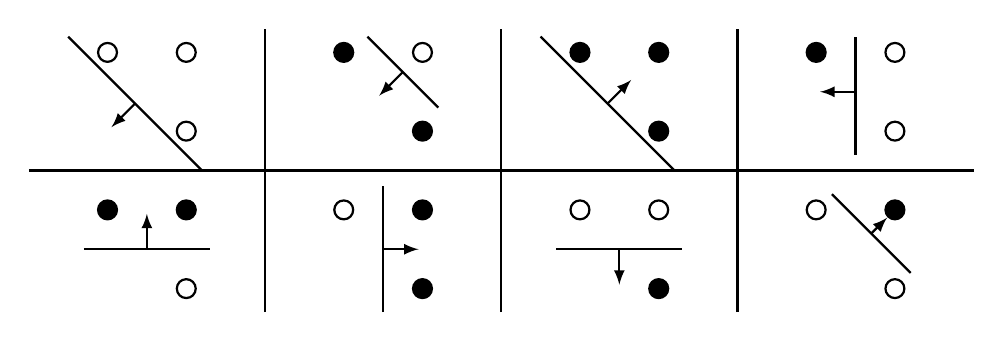
\begin{tikzpicture}[thick, >={latex}]
		\draw (0, 5.5) circle (0.12);
		\draw (1, 5.5) circle (0.12);
		\draw (1, 4.5) circle (0.12);
		\draw (4, 5.5) circle (0.12);
		\draw (10, 5.5) circle (0.12);
		\draw (10, 4.5) circle (0.12);
		\draw (1, 2.5) circle (0.12);
		\draw (3, 3.5) circle (0.12);
		\draw (6, 3.5) circle (0.12);
		\draw (7, 3.5) circle (0.12);
		\draw (9, 3.5) circle (0.12);
		\draw (10, 2.5) circle (0.12);
		
		\draw[fill] (3, 5.5) circle (0.12);
		\draw[fill] (4, 4.5) circle (0.12);
		\draw[fill] (6, 5.5) circle (0.12);
		\draw[fill] (7, 5.5) circle (0.12);
		\draw[fill] (7, 4.5) circle (0.12);
		\draw[fill] (9, 5.5) circle (0.12);
		\draw[fill] (0, 3.5) circle (0.12);
		\draw[fill] (1, 3.5) circle (0.12);
		\draw[fill] (4, 3.5) circle (0.12);
		\draw[fill] (4, 2.5) circle (0.12);
		\draw[fill] (7, 2.5) circle (0.12);
		\draw[fill] (10, 3.5) circle (0.12);
		
		\draw (-1, 4) -- (11, 4);
		\draw (2, 2.2) -- (2, 5.8);
		\draw (5, 2.2) -- (5, 5.8);
		\draw (8, 2.2) -- (8, 5.8);
		
		\draw (-0.5, 5.7) -- (1.2, 4);
		\draw[->] (0.35, 4.85) -- (0.05, 4.55);
		\draw (3.3, 5.7) -- (4.2, 4.8);
		\draw[->] (3.75, 5.25) -- (3.45, 4.95);
		\draw (5.5, 5.7) -- (7.2, 4);
		\draw[->] (6.35, 4.85) -- (6.65, 5.15);
		\draw (9.5, 4.2) -- (9.5, 5.7);
		\draw[->] (9.5, 5) -- (9.05, 5);
		\draw (-0.3, 3) -- (1.3, 3); 
		\draw[->] (0.5, 3) -- (0.5, 3.45);
		\draw (3.5, 2.2) -- (3.5, 3.8);
		\draw[->] (3.5, 3) -- (3.95, 3);
		\draw (5.7, 3) -- (7.3, 3); 
		\draw[->] (6.5, 3) -- (6.5, 2.55);
		\draw (9.2, 3.7) -- (10.2, 2.7);
		\draw[->] (9.7, 3.2) -- (9.9, 3.4);
	\end{tikzpicture}
\end{center}

Avec $d_\Hyp$ on peut obtenir une borne pour $\trisk(h)$.

\PROP[ (Borne de généralisation dans le cas infini)] {
	Avec probabilité $1 - \delta$, on a pour tout $h$ dans $\Hyp$ :
	$$ \trisk(h) \leqslant \erisk(h) + \sqrt{\dfrac{d_\Hyp \left( \ln \frac{2 m}{d_\Hyp} + 1 \right) + ln \frac{4}{\delta}}{m}} $$
	\vspace{-5mm}
}

Au lieu d'utiliser la dimension VC, on peut aussi utiliser la complexité de Rademacher.

\DEF{
	La \textbf{complexité empirique de Rademacher} de $\Hyp$ est :
	$$ Rad_m(\Hyp, S) = \E \left( \sup_{h \in \Hyp} \left| \frac{1}{m} \sum_{i = 1}^m \sigma_i h(z_i) \right| \right) $$
	Où $\sigma_1, \dots, \sigma_m$ sont $m$ variables de Rademacher i.i.d avec $\Pp(\sigma_i = 1) = \Pp(\sigma_i = -1) = \frac{1}{2}$.
}

\PROP[ (Borne de convergence uniforme avec la complexité de Rademacher)] {
	Avec probabilité $1 - \delta$, on a pour tout $h$ dans $\Hyp$ : \vspace{-3mm}
	$$ \trisk(h) \leqslant \erisk(h) + 2 Rad_m(\Hyp, S) + \sqrt{\dfrac{4}{m} ln \left( \dfrac{2}{\delta} \right)} $$
	\vspace{-5mm}
}

\subsubs{Stabilité uniforme}

On veut réduire la variance sans modifier le biais. On va voir qu'avoir une faible variance est équivalent à avoir une grande stabilité. Intuitivement un algorithme est stable si pour de petits changements dans l'ensemble d'entraînement, la sortie $h$ de l'algorithme varie peu.

Dans la définition qui suit, on utilise les notations suivantes :
\begin{itemize}
	\item $S^{\setminus i} = \{ z_1, \dots, z_{i-1}, z_{i+1}, \dots, z_m \}$ pour l'ensemble $S$ sans le $i$-ème exemple.
	\item $S^{i} = \{ z_1, \dots, z_{i-1}, z_i^\prime, z_{i+1}, \dots, z_m \}$ pour l'ensemble $S$ dont le $i$-ème exemple est remplacé par une valeur aléatoire suivant la loi $\dist$.
\end{itemize}

\DEF{
	Un algorithme $L$ a une \textbf{stabilité uniforme} $\dfrac{\beta}{m}$ respectivement à une fonction de perte $l$ si :
	$$ \forall S, \, \forall i \in \{1, ..., m\} \, \sup_z \left| l(h_S, z) - l(h_{S^{\setminus i}}, z) \right| \leqslant \dfrac{\beta}{m} $$
	\vspace{-5mm}
}

Par inégalité triangulaire on obtient :
$$ \forall S, \, \forall i \in \{1, ..., m\} \, \sup_z \left| l(h_S, z) - l(h_{S^{i}}, z) \right| \leqslant 2 \dfrac{\beta}{m} $$


\PROP[ (Borne de généralisation utilisant la stabilité uniformes)] {
	Soit $S$ un ensemble d'entraînement de taille $m$. Alors pour tout algorithme $L$ de stabilité uniforme $\dfrac{\beta}{m}$ respectivement à une fonction de perte $l$ bornée par $M$, on a avec probabilité $1 - \delta$ : \vspace{-3mm}
	$$ \trisk(h_S) \leqslant \erisk(h_S) + 2 \dfrac{\beta}{m} + (4 \beta + M) \sqrt{\dfrac{\ln \frac{1}{\delta}}{2m}} $$
	\vspace{-5mm}
}

Pour la démonstration, on a besoin du théorème suivant :

\PROP[ (McDiarmid)]{
	Soit $F : \Z^m \rightarrow \R$ une fonction pour laquelle il existe des constantes $c_1, ..., c_m$ tel que \vspace{-2mm}
	$$ \sup_{S \in \Z^m, z_i^\prime \in \Z} \left| F(S) - F(S^i) \right| \leqslant c_i $$
	\vspace{-2mm} Alors \vspace{-2mm}
	$$ \Pp(F(S) - \E_S[F(S)] \geqslant \gamma) \leqslant \exp \left( \dfrac{- 2 \gamma^2}{\sum_{i = 1}^m c_i^2} \right) $$
	\vspace{-5mm}
}

\dem
Comme l'espérance est inférieure au $\sup$ d'une variable aléatoire, on a :
$$ \begin{array}{llc}
	| \trisk(h_S) - \trisk(h_{S^{\setminus i}}) | & = & \left| \E_z[l(h_S, z)] - \E_z[l(h_{S^{\setminus i}}, z)] \right| \\
	 & \leqslant & \dfrac{\beta}{m}
\end{array} $$
On utilise alors l'inégalité triangulaire pour déduire :
$$ \begin{array}{llc}
| \trisk(h_S) - \trisk(h_{S^{i}}) | & = & | \trisk(h_S) - \trisk(h_{S^{\setminus i}}) | + | \trisk(h_{S^i}) - \trisk(h_{S^{\setminus i}}) | \\
& \leqslant & 2 \dfrac{\beta}{m}
\end{array} $$
On passe ensuite au risque empirique :
$$ \begin{array}{lll}
	| \erisk(h_S) - \erisk(h_{S^{\setminus i}}) |
	 & = & \left| \displaystyle \dfrac{1}{m} \sum_{j \neq i} \left( l(h_S, z_j) - l(h_{S^{\setminus i}}, z_j) \right) + \dfrac{1}{m} l(h_S, z_i) \right| \\
	 & \leqslant & \displaystyle \dfrac{1}{m} \sum_{j \neq i} \left| l(h_S, z_j) - l(h_{S^{\setminus i}}, z_j) \right| + \dfrac{1}{m} | l(h_S, z_i) | \\
	 & \leqslant & \dfrac{\beta}{m} + \frac{M}{m}
\end{array}$$
Toujours avec l'inégalité triangulaire, on obtient ensuite :
$$ | \erisk(h_S) - \erisk(h_{S^{i}}) | \leqslant 2 \dfrac{\beta}{M} + 2 \dfrac{M}{m} $$
Cependant on peut faire un peu mieux :
$$ \begin{array}{lll}
	| \erisk(h_S) - \erisk(h_{S^{i}}) |
	& \leqslant & \displaystyle \dfrac{1}{m} \sum_{j \neq i} \left| l(h_S, z_j) - l(h_{S^{ i}}, z_j) \right| + \dfrac{1}{m} | l(h_S, z_i) - l(h_S, z_i^\prime) | \\
	& \leqslant & 2 \dfrac{\beta}{m} + \frac{M}{m}
\end{array}$$
On considère alors la fonction $F = \trisk - \erisk$ pour utiliser le théorème de McDiarmid :
$$ \begin{array}{lll}
	| F(S) - F(S^i) |
	& = & | (\trisk(h_S) - \erisk(h_S)) - (\trisk(h_{S^i}) - \erisk(h_{S^i}) | \\
	& \leqslant & | \trisk(h_S) - \trisk(h_{S^i}) | + | \erisk(h_S) - \erisk(h_{S^i}) | \\
	& \leqslant & 4 \dfrac{\beta}{m} + \dfrac{M}{m} = c_i
\end{array} $$
D'après le théorème de McDiarmid on a donc :
$$ \Pp(F(S) - \E_S[F(S)] \geqslant \gamma) \leqslant \exp \left( \dfrac{- 2 \gamma^2}{\sum_{i = 1}^m c_i^2} \right) $$
Il nous faut désormais calculer l'espérance de $F(S)$.
$$ \begin{array}{lll}
	\E_S[\trisk(h_S) - \erisk(h_S)]
	& = & \E_S[\trisk(h_S)] - \E_S[\erisk(h_S)] \\
	& = &\displaystyle \E_{S, z \sim \dist}[l(h_S, z)] - \dfrac{1}{m} \sum_{j = 1}^m \E_S[l(h_S, z_j)] \\
	& = & \displaystyle \E_{S, z \sim \dist}[l(h_S, z)] - \dfrac{1}{m} \sum_{j = 1}^m \E_{S, z_j^\prime \sim \dist}[l(h_{S^j}, z_j^\prime)] \\
	& = & \E_{S, z_j^\prime \sim \dist}[l(h_S, z_j^\prime)-l(h_{S^j}, z_j^\prime)] \\ \vspace{1mm}
	& \leqslant & \displaystyle \E_{S, z_j^\prime \sim \dist} \left[ | l(h_S, z_j^\prime)-l(h_{S^j}, z_j^\prime) | \right] \\
	& \leqslant & \displaystyle \E_{S, z_j^\prime \sim \dist} \left[ | l(h_S, z_j^\prime)-l(h_{S^{\setminus j}}, z_j^\prime) | \right] + \E_{S, z_j^\prime \sim \dist} \left[ | l(h_{S^{\setminus j}}, z_j^\prime)-l(h_{S^j}, z_j^\prime) | \right] \\
	& \leqslant & 2 \dfrac{\beta}{m}
\end{array} $$
Cela nous donne finalement :
$$ \Pp \left( \trisk - \erisk \geqslant \gamma + 2 \dfrac{\beta}{m} \right) \leqslant \exp \left( \dfrac{- 2 m \gamma^2}{(4 \beta + M)^2} \right) $$
Et en prenant $\gamma$ tel que la partie de droite soit $1 - \delta$ on obtient bien :
$$ \trisk(h_S) \leqslant \erisk(h_S) + 2 \dfrac{\beta}{m} + (4 \beta + M) \sqrt{\dfrac{\ln \frac{1}{\delta}}{2m}} $$
\findem

Maintenant il nous faut savoir comment trouver $\beta$.

\PROP[ (Stabilité avec régularisation)]{
	Si notre apprentissage est de la forme :
	$$ \min_{h \in \Hyp} \dfrac{1}{m} \sum_i l(h, z_i) + \lambda \| h \|^2 $$
	Alors si $l$ est $\sigma$-admissible, c'est à dire que $x \mapsto l(h(x), y)$ est $\sigma$-lipschitzienne pour tout $h$ et tout $y$, on a :
	$$ \beta \leqslant \dfrac{\sigma^2}{2 \lambda} $$
	\vspace{-5mm}
}

\subsubs{Robustesse algorithmique}

\DEF{
	Un algorithme $L$ est $\bm{(K, \epsilon(.))}$\textbf{-robuste} pour $K \in \N$ et $\epsilon : \mathcal{P}(\Z) \rightarrow \R$ si pour tout $S \in \mathcal{P}(\Z)$, $\Z$ peut être partitionné en $K$ sous-ensembles $\{ C_i \}_{i = 1}^K$ tel que :
	$$ \forall i \in [K], \, \forall z, z' \in C_i, \, z \in S \Rightarrow |l(h_S, z) - l(h_S, z')| \leqslant \epsilon(S) $$
	\vspace{-5mm}
}

\PROP[ (borne de robustesse)]{
	Si un algorithme est $(K, \epsilon(.))$-robuste, alors avec probabilité $1 - \delta$ :
	$$ \trisk(h_S) \leqslant \erisk(h_S) + \epsilon(S) + \sqrt{\dfrac{2K \ln 2 + 2 \ln(1/\delta)}{m}} $$
	\vspace{-5mm}
}

\subs{Choix du modèle}

\renewcommand{\trisk}{\mathcal{R}}
\renewcommand{\erisk}{\hat{\mathcal{R}}}

Les bornes de généralisation PAC ne sont pas vraiment utilisables car elles sont vraiment pessimistes. Une idée peut être la validation croisée qui permet de mesurer la généralisation d'un modèle après entraînement.

\begin{center}
	\begin{algorithm}[H]
		\KwIn{Un algorithme d'apprentissage $L$ et un ensemble d'apprentissage $S$}
		\KwOut{une estimation $\erisk_2(h)$ de $\trisk(h)$}
		\vspace{3mm}
		Séparer $S$ en $k$ sous-ensembles $S_1, \dots, S_k$\;
		\For{$i=1$ à $k$}{
			Exécuter $L$ sur $S \setminus S_i$ pour obtenir un classifieur $h_i$;
		}
		Déduire l'estimation du risque $\erisk_2(h) = \frac{1}{k} \sum_{i = 1}^k \erisk_2(h_i)$ où $\erisk_2(h_i)$ est l'erreur de $h_i$ sur $S_i$\;
		\vspace{3mm}
		\caption{Algorithme de $k$-validation croisée}
	\end{algorithm}
\end{center}

Avec cet algorithme on peut alors comparer différent algorithmes d'apprentissage.

\exe
\begin{center}
	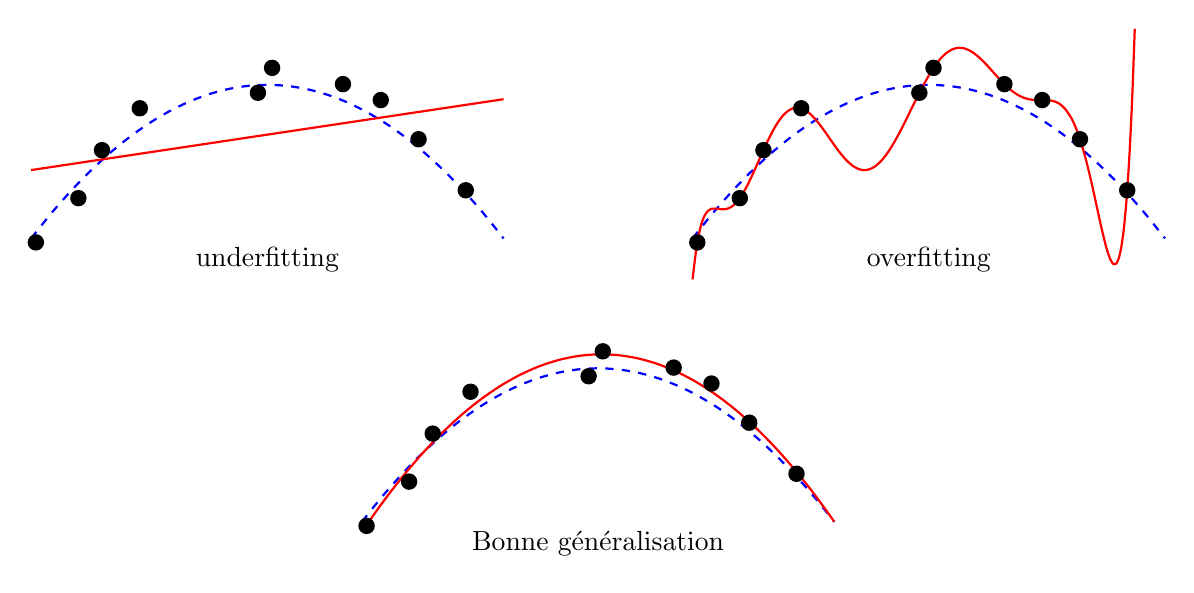
\begin{tikzpicture}[thick, scale=0.6]
		\draw[domain=0:10, smooth, variable=\x, blue, dashed]
			plot ({\x}, {-0.55 + 1.3 * \x * (1 - 0.1 * \x)});
		\draw[domain=0:10, smooth, variable=\x, red]
			plot ({\x}, {0.895863 + 0.14997759 * \x)});
		\draw[circle, fill] (0.1, -0.6349920559756366) circle(0.15);
		\draw[circle, fill] (1.0, 0.30147401369268423) circle(0.15);
		\draw[circle, fill] (1.5, 1.3173171840454918) circle(0.15);
		\draw[circle, fill] (2.3, 2.2037856155666598) circle(0.15);
		\draw[circle, fill] (4.8, 2.53199171235714) circle(0.15);
		\draw[circle, fill] (5.1, 3.0593432681003296) circle(0.15);
		\draw[circle, fill] (6.6, 2.7147727490453817) circle(0.15);
		\draw[circle, fill] (7.4, 2.377546686262505) circle(0.15);
		\draw[circle, fill] (8.2, 1.5487114646843132) circle(0.15);
		\draw[circle, fill] (9.2, 0.46764396433128286) circle(0.15);
		\node at (5, -1) {underfitting};
		
		\draw[domain=0:10, smooth, variable=\x, blue, dashed]
			plot ({\x+14}, {-0.55 + 1.3 * \x * (1 - 0.1 * \x)});
		\draw[domain=0:2, smooth, variable=\x, red]
			plot ({\x+14}, {-1.41950554e+00 + \x * (1.00967400e+01 + \x * (-2.53146666e+01 +
				\x * (2.96771161e+01 + \x * (-1.74688908e+01 + \x * (5.69941439e+00 +
				\x * (-1.08044823e+00 + \x * (1.18525383e-01 + \x * (-6.98156850e-03 +
				\x * 0.000170922685)))))))});
		\draw[domain=-1:2, smooth, variable=\x, red]
			plot ({\x+17}, {1.42484270e+00 + \x * (-1.40170537e+00 + \x * (3.40897007e-01 +
			\x * (1.03657493e+00 + \x * (-1.83881811e-01 + \x * (-1.59051020e-01 +
			\x * (3.68822015e-02 + \x * (6.34668910e-03 + \x * (-2.36665600e-03 +
			\x * 1.70922685e-04)))))))});
		\draw[domain=-1:2, smooth, variable=\x, red]
		plot ({\x+20}, {3.33547340e+00 + \x * (-7.96494283e-01 + \x * (-8.55389836e-01 +
			\x * (6.85820570e-01 + \x * (2.21442569e-01 + \x * (-1.29594094e-01 +
			\x * (-3.85819884e-02 + \x * (4.92589522e-03 + \x * (2.24825651e-03 +
			\x * 1.70922685e-04)))))))});
		\draw[domain=-1:0.36, smooth, variable=\x, red]
			plot ({\x+23}, {-1.02813387e+00 + \x * (2.33112518e+00 + \x * (1.98927127e+01 +
				\x * (2.58711983e+01 + \x * (1.57048589e+01 + \x * (5.25072508e+00 +
				\x * (1.01907510e+00 + \x * (1.14263001e-01 + \x * (6.86316901e-03 +
				\x * 1.70922685e-04)))))))});
		\draw[circle, fill] (14.1, -0.6349920559756366) circle(0.15);
		\draw[circle, fill] (15.0, 0.30147401369268423) circle(0.15);
		\draw[circle, fill] (15.5, 1.3173171840454918) circle(0.15);
		\draw[circle, fill] (16.3, 2.2037856155666598) circle(0.15);
		\draw[circle, fill] (18.8, 2.53199171235714) circle(0.15);
		\draw[circle, fill] (19.1, 3.0593432681003296) circle(0.15);
		\draw[circle, fill] (20.6, 2.7147727490453817) circle(0.15);
		\draw[circle, fill] (21.4, 2.377546686262505) circle(0.15);
		\draw[circle, fill] (22.2, 1.5487114646843132) circle(0.15);
		\draw[circle, fill] (23.2, 0.46764396433128286) circle(0.15);
		\node at (19, -1) {overfitting};
		
		\draw[domain=0:10, smooth, variable=\x, blue, dashed]
			plot ({\x+7}, {-6.55 + 1.3 * \x * (1 - 0.1 * \x)});
		\draw[domain=0:10, smooth, variable=\x, red]
			plot ({\x+7}, {-6.76178277 + \x * (1.48142299 - 0.14599194 * \x)});
		\draw[circle, fill] (7.1, -6.634992055975637) circle(0.15);
		\draw[circle, fill] (8.0, -5.698525986307316) circle(0.15);
		\draw[circle, fill] (8.5, -4.682682815954508) circle(0.15);
		\draw[circle, fill] (9.3, -3.7962143844333402) circle(0.15);
		\draw[circle, fill] (11.8, -3.46800828764286) circle(0.15);
		\draw[circle, fill] (12.1, -2.9406567318996704) circle(0.15);
		\draw[circle, fill] (13.6, -3.2852272509546183) circle(0.15);
		\draw[circle, fill] (14.4, -3.622453313737495) circle(0.15);
		\draw[circle, fill] (15.2, -4.451288535315687) circle(0.15);
		\draw[circle, fill] (16.2, -5.532356035668717) circle(0.15);
		\node at (12, -7) {Bonne généralisation};		
	\end{tikzpicture}
\end{center}

On cherche un modèle sous forme de polynôme.
$$ h_{\theta^{(1)}}(x) = \theta^{(1)}_0 + \theta^{(1)}_1 x $$
$$ h_{\theta^{(2)}}(x) = \theta^{(2)}_0 + \theta^{(2)}_1 x + \theta^{(2)}_2 x^2 $$
$$ \dots $$
$$ h_{\theta^{(10)}}(x) = \theta^{(10)}_0 + \theta^{(10)}_1 x + \dots + \theta^{(10)}_{10} x^{10} $$
On souhaite savoir quel degré $d^* \in \{ 1, ..., 10 \}$ on doit choisir. Ici $\theta$ est l'ensemble de paramètres à apprendre et $d^*$ peut être vu comme un paramètre extra à régler. \\

On peut alors séparer notre ensemble d'entraînement en deux sous-ensembles $S = Train \cup Test$. Le degré optimal ensuite être obtenu en apprenant les paramètres $\theta^{1}, \dots, \theta^{(10)}$ grâce au sous-ensemble $Train$ puis en sélectionnant le modèle avec la plus petite erreur sur le sous-ensemble $Test$.

\paragraph{Cependant !} On ne peut pas réutiliser l'ensemble $Test$ pour estimer le vrai risque. En effet cela ne serait pas équitable car on a choisi le paramètre $d^*$ de sorte à minimiser l'erreur sur $Test$. L'erreur de généralisation obtenue sur cette ensemble est donc bien trop optimiste.	On doit donc finalement séparé notre ensemble d'entraînement en trois sous-ensembles :
\begin{itemize}
	\item \textbf{L'ensemble d'entraînement} pour apprendre les paramètres $\theta^{(1)}, \dots, \theta^{(10)}$.
	\item \textbf{L'ensemble de validation} pour choisir le meilleur paramètre $d^*$.
	\item \textbf{L'ensemble de teste} pour estimer l'erreur de généralisation de $h_{\theta^{(d^*)}}$.
\end{itemize}
Si $\erisk(h)$ est l'erreur obtenue sur l'ensemble d'entraînement alors on peut voir $\erisk(h)$ comme le biais de $h$. De même si $\vrisk(h)$ est l'erreur obtenue sur l'ensemble de validation alors on peut voir $V = \vrisk(h) - \erisk(h)$ comme la variance de $h$.

\exe
On obtient les résultats suivants :
\begin{itemize}
	\item Erreur d'entraînement : $1\%$
	\item Erreur de validation : $11\%$
\end{itemize}
Cela veut dire que la variance est bien plus élevée que le biais. On peut donc corriger cela en entraînant l'algorithme sur une plus grand ensemble d'entraînement. \\
En revanche si on obtient les résultats suivants :
\begin{itemize}
	\item Erreur d'entraînement : $15\%$
	\item Erreur de validation : $16\%$
\end{itemize}
Cela veut dire que c'est le biais qui est élevé par rapport à la variance. Il faut donc augmenter l'expressivité de notre modèle.